\documentclass[12pt]{beamer}
\usepackage[utf8]{inputenc}
\usepackage[spanish]{babel}
\usepackage{color}
\usepackage{hyperref}
\usepackage{amsmath}
\usepackage{amsthm}
\usepackage{multicol}
\usepackage{graphicx}
\usepackage{tikz}
\usepackage[autostyle,spanish=mexican]{csquotes}
%\usepackage[sfdefault]{roboto}  %% Option 'sfdefault' only if the base font of the document is to be sans serif
\renewcommand{\arraystretch}{1.5}
\renewcommand{\rmdefault}{cmr}% cmr = Computer Modern Roman
\usefonttheme[onlymath]{serif}

\newcommand{\python}{\texttt{python}}
\newcommand{\textoazul}[1]{\textcolor{blue}{#1}}
\newcommand{\azulfuerte}[1]{\textcolor{blue}{\textbf{#1}}}
\newcounter{saveenumi}
\newcommand{\seti}{\setcounter{saveenumi}{\value{enumi}}}
\newcommand{\conti}{\setcounter{enumi}{\value{saveenumi}}}

\linespread{1.5}
\beamertemplatenavigationsymbolsempty
\usefonttheme{professionalfonts}
\usefonttheme{serif}
\DeclareGraphicsExtensions{.pdf,.png,.jpg}
\renewcommand {\arraystretch}{1.25}
\mode<presentation>
{
  \usetheme{Warsaw}
  \setbeamertemplate{headline}{}
  %\useoutertheme{infolines}
  \useoutertheme{default}
  \setbeamercovered{invisible}
  % or whatever (possibly just delete it)
  \setbeamertemplate{section in toc}[sections numbered]
  \setbeamertemplate{subsection in toc}[subsections numbered]
  \setbeamertemplate{subsection in toc}{\leavevmode\leftskip=3.2em\rlap{\hskip-2em\inserttocsectionnumber.\inserttocsubsectionnumber}\inserttocsubsection\par}
  \setbeamercolor{section in toc}{fg=blue}
  \setbeamercolor{subsection in toc}{fg=blue}
  \setbeamercolor{frametitle}{fg=yellow}

  \setbeamertemplate{footline} 
{
  \leavevmode%
  \hbox{%
  \begin{beamercolorbox}[wd=.333333\paperwidth,ht=2.25ex,dp=1ex,center]{author in head/foot}%
    \usebeamerfont{author in head/foot}\insertsection
  \end{beamercolorbox}%
  \begin{beamercolorbox}[wd=.333333\paperwidth,ht=2.25ex,dp=1ex,center]{title in head/foot}%
    \usebeamerfont{title in head/foot}\textcolor{yellow}{\insertsubsection}
  \end{beamercolorbox}%
  \begin{beamercolorbox}[wd=.333333\paperwidth,ht=2.25ex,dp=1ex,right]{date in head/foot}%
    \usebeamerfont{date in head/foot}\insertshortdate{}\hspace*{2em}
    \insertframenumber{} / \inserttotalframenumber\hspace*{2ex} 
  \end{beamercolorbox}}%
  \vskip0pt%
}
}
\makeatother

\makeatletter
\patchcmd{\beamer@sectionintoc}
  {\vfill}
  {\vskip\itemsep}
  {}
  {}
\makeatother
\title{Cálculo de raíces con funciones de \python{}}
\subtitle{Tema 2 - Operaciones matemáticas básicas}
\author{M. en C. Gustavo Contreras Mayén}
\date{\today}
\institute{Facultad de Ciencias - UNAM}
\titlegraphic{\includegraphics[width=1.75cm]{Imagenes/escudo-facultad-ciencias}\hspace*{4.75cm}~%
   \includegraphics[width=1.75cm]{Imagenes/escudo-unam}
}
\begin{document}
\maketitle
\fontsize{14}{14}\selectfont
\spanishdecimal{.}
\section*{Contenido}
\frame{\tableofcontents[currentsection, hideallsubsections]}
\section{La librería \texttt{scipy.optimize}}
\frame{\tableofcontents[currentsection, hideothersubsections]}
\subsection*{Contenido del paquete}
\begin{frame}
\frametitle{Contenido del paquete \texttt{scipy.optimize}}
La librería \funcionazul{scipy.optimize} proporciona un conjunto de funciones para:
\setbeamercolor{item projected}{bg=blue!70!black,fg=yellow}
\setbeamertemplate{enumerate items}[circle]
\begin{enumerate}[<+->]
\item Minimizar (o maximizar) funciones.
\item Soluciones de problemas no lineales.
\item Programación lineal.
\item Cálculo de mínimos cuadrados restringidos y no lineales.
\item Ajuste de curvas.
\item \textcolor{red}{Búsqueda de raíces.}
\end{enumerate}
\end{frame}
\begin{frame}
\frametitle{Funciones en \texttt{optimize}}
En la librería \funcionazul{scipy.optimize} encontraremos al menos $8$ funciones para el cálculo de raíces.
\\
\bigskip
Nos enfocaremos a dos de ellas y que ya vimos anteriormente: el método de bisección y el de Newton-Raphson.
\end{frame}
\begin{frame}
\frametitle{Recomendación}
Es conveniente revisar la teoría correspondiente de las otras técnicas que se incluyen en la librería \funcionazul{scipy.optimize}: el método de Ridder, el método de Brent, el algoritmo TOMS 748.
\\
\bigskip
De esta manera, ya sería posible ocupar esas funciones para resolver un problema en particular.
\end{frame}
\section{La función \texttt{bisect}}
\frame{\tableofcontents[currentsection, hideothersubsections]}
\subsection{La función bisect}
\begin{frame}[fragile]
\frametitle{La función \texttt{bisect}}
La sintaxis mínima para esta función es la siguiente:
\\
\verb|scipy.optimize.bisect(f, a, b)|
\\
Encuentra la raíz de una función \textoazul{f}, en un intervalo dado $(a, b)$.
\end{frame}
\begin{frame}[fragile]
\frametitle{La función \texttt{bisect}}
Es importante señalar que la función requere que los valores de $f(a)$ y $f (b)$ deben de tener signos contrarios.
\\
\bigskip
Es un método lento, pero seguro.
\end{frame}
\begin{frame}[fragile]
\frametitle{El valor de regreso}
La función \funcionazul{bisect} devuelve un valor $x_{0}$ que corresponde al valor de la raíz.
\\
\bigskip
\pause
Existen otros argumentos sobre el número de iteraciones, la tolerancia permitida, etc., es conveniente que revises la documentación para que los conozcas y determines en un momento dado, si modificas alguno.
\end{frame}
\begin{frame}[fragile]
\frametitle{Ejemplo de uso}
Usando la función \funcionazul{bisect} calcula las raíces de $f(x)$, tal que:
\begin{align*}
f(x) =  x^{2} - 1
\end{align*}
\end{frame}
\begin{frame}
\frametitle{Graficamos la función}
Como es costumbre, graficamos la función para darnos una idea preliminar del comportamiento de $f(x)$:
\begin{figure}[h!]
    \centering
    \includegraphics[scale=0.4]{Imagenes/raices_scipy_bisect_01.eps}
    \caption{Gráfica general de la función $f(x)$}
\end{figure}
\end{frame}
\begin{frame}
\frametitle{Apoyo para los intervalos}
Para determinar los intervalos en donde se encuentran las raíces, debemos de utilizar la función \funcionazul{buscaraiz}, recuerda que todo paso se debe de justificar debidamente, el ojímetro debe de quedar guardado.
\end{frame}
\begin{frame}[allowframebreaks, fragile]
\frametitle{Código}
\begin{lstlisting}[caption=Código para el cálculo de la raíz con \texttt{optimize.bisect}, style=codigopython]
from scipy import optimize

def f(x):
    return (x**2 - 1)

aA_1_B, bA_1_B = buscaraiz(f, inicio, final, dx)

raizA_1_B = optimize.bisect(f, aA_1_B, bA_1_B)

print('La raiz esta en x = {0:1.6f}'.format(raizA_1_B))
\end{lstlisting}
\end{frame}
\begin{frame}
\frametitle{Gráfica con los resultados}
Deberás de incorporar la rutina de graficación para mostrar los resultados:
\begin{figure}[h!]
    \centering
    \includegraphics[scale=0.4]{Imagenes/raices_scipy_bisect_02.eps}
    \caption{Gráfica con las raíces de la función $f(x)$}
\end{figure}
\end{frame}
\subsection{La función \texttt{Newton}}
\begin{frame}[fragile]
\frametitle{La función \texttt{Newton}}
La función que utiliza el método de Newton-Raphson que hemos discutido anteriormente, está incluida en la librería \funcionazul{scipy.optimize} y es la función \funcionazul{Newton}, que tiene la sintaxis:
\\
\bigskip
\verb|scipy.optimize.newton(func, x0, fprime=None)|
\end{frame}
\begin{frame}[fragile]
\frametitle{La función \texttt{Newton}}
Esta función encuentra un cero usando el método de Newton-Raphson o el método de la secante.
\\
\bigskip
Encuentra un cero de la función \funcionazul{func} cercano a un punto inicial $x_{0}$
\end{frame}
\begin{frame}[fragile]
\frametitle{La función \texttt{Newton}}
Se utiliza el método de Newton-Raphson si se proporciona la derivada de la función: \funcionazul{fprime}, en caso contrario, se utiliza el método de la secante.
\end{frame}
\begin{frame}
\frametitle{Ejemplo para resolver}
Usando la función \textoazul{optimize.newton} calcula la raíz de $f(x)$:
\begin{align*}
f(x) = x^{3} - 1
\end{align*}
Graficamos la función para ver su comportamiento (la raíz que se obtenga es de multiplicidad 3, ya sea con métodos construidos o con funciones de \python, ¿cómo podríamos reportar estas raíces múltiples?)
\end{frame}
\begin{frame}
\frametitle{Gráfica de la función}
\begin{figure}[h!]
    \centering
    \includegraphics[scale=0.5]{Imagenes/raices_scipy_newton_01.eps}
    \caption{Comportamiento general de la función $f(x)$}
\end{figure}
\end{frame}
\begin{frame}[allowframebreaks, fragile]
\frametitle{Código para el ejercicio}
\begin{lstlisting}[caption=Código que usa \texttt{optimize.newton} pero sin la derivada de la función, style=codigopython]
from scipy import optimize

def f(x):
    return (x**3 - 1)

raiz = optimize.newton(f, 1.5)

print('La raiz esta en x = {0:}'.format(raiz))
\end{lstlisting}
\end{frame}
\begin{frame}
\frametitle{Resultado gráfico}
\begin{figure}[h!]
    \centering
    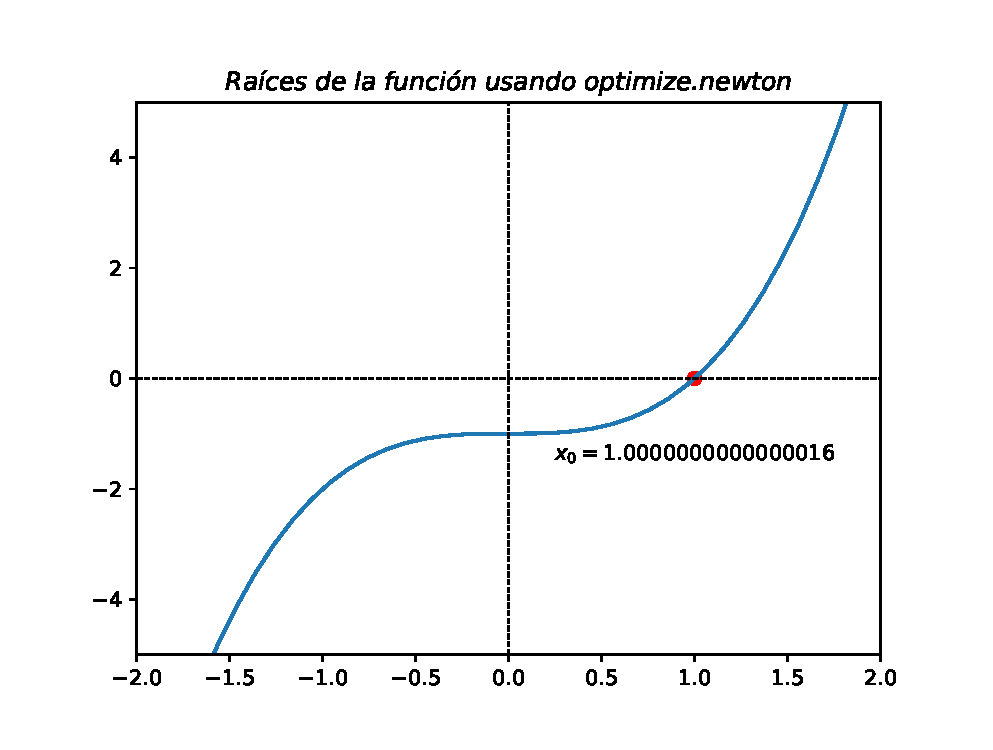
\includegraphics[scale=0.5]{Imagenes/raices_scipy_newton_02.eps}
    \caption{Raíz de la función $f(x)$}
\end{figure}
\end{frame}
\begin{frame}
\frametitle{Consideraciones}
En el código anterior, no se ha proporcionado la derivada de la función $f(x)$ por lo que el método que se ocupa es el método de la secante.
\end{frame}
\begin{frame}
\frametitle{Incluyendo la derivada de la función}
Una forma \enquote{económica} para incorporar la derivada, es usando funciones \funcionazul{lambda}, que como ya sabemos, se ocupan una sola vez y no es necesario declararlas con la palabra reservada \funcionazul{def}.
\end{frame}
\begin{frame}[allowframebreaks, fragile]
\frametitle{Código para el ejercicio}
\begin{lstlisting}[caption=Código que usa \texttt{optimize.newton} con la derivada de la función, style=codigopython]
from scipy import optimize

def f(x):
    return (x**3 - 1)

raiz = optimize.newton(f, 1.5, fprime=lambda x: 3 * x**2)

print('La raiz esta en x = {0:}'.format(raiz))
\end{lstlisting}
\end{frame}
\begin{frame}
\frametitle{Conclusiones del método \texttt{newton}}
En este caso particular, el resultado en ambos casos el valor de la raíz es el mismo.
\\
\bigskip
Habrá que revisar con detenimiento el planteamiento del problema, para seleccionar debidamente el tipo de método que se vaya a requerir.
\end{frame}
\section{Aplicaciones}
\frame{\tableofcontents[currentsection, hideothersubsections]}
\subsection{Ejercicio 1 - La ecuación de Kepler}
\begin{frame}
\frametitle{La ecuación de Kepler}
La ecuación de Kepler juega un papel central en la mecánica celeste clásica, porque permite el cálculo de las posiciones angulares para los objetos en órbita.
\\
\bigskip
Para una órbita elíptica, relaciona la anomalía media $M$, la anomalía excéntrica $E$ y la excentricidad $e$, de la siguiente forma:
\end{frame}
\begin{frame}
\frametitle{La ecuación de Kepler}
\begin{align}
M = E - e \, \sin E
\label{eq:ecuacion_6_58}
\end{align}
donde
\begin{align*}
e = \sqrt{1 - \dfrac{b^{2}}{a^{2}}}
\end{align*}
donde $a > b$ son los semiejes.
\end{frame}
\begin{frame}
\frametitle{La anomalía media}
Los astrónomos definen las \enquote{anomalías} como posiciones angulares: la anomalía media $M$ es la posición angular del objeto en una órbita circular ficticia.
\end{frame}
\begin{frame}
\frametitle{La anomalía media}
Suponiendo una velocidad angular constante, $M$ puede estar relacionada con el período de tiempo desde el paso a través del perihelio:
\begin{align}
M = \dfrac{2 \, \pi}{T} \, (t - t_{0})
\label{eq:ecuacion_6_59}
\end{align}
donde $T$ es el período orbital y $t_{0}$ es el tiempo en donde el objeto cruza el perihelio.
\end{frame}
\begin{frame}
\frametitle{Datos para el cometa Halley}
Consideremos el cometa Halley, con los siguientes datos:
\begin{table}
\centering
\begin{tabular}{c c}
Parámetro & Valor \\ \hline
$e$ & $0.9672671$ \\ \hline
$T$ & $75.9600$ años \\ \hline
$t_{0}$ & $1986.1113$ años\footnote{en 9 de febrero de 1986} \\ \hline
\end{tabular}
\end{table}
\end{frame}
\begin{frame}
\frametitle{Problemas a resolver}
\setbeamercolor{item projected}{bg=blue!70!black,fg=yellow}
\setbeamertemplate{enumerate items}[circle]
\begin{enumerate}[<+->]
\item Calcula la anomalía excéntrica $E$ del cometa Halley para el 1 de abril de 1986, para $t = 1986.2491$.
Para resolver este punto, grafiquemos la función
\begin{align}
f(E) = E - e \, \sin E - M
\label{eq_ecuacion_6_60}
\end{align}
para $E \in [0,1]$, debemos asegurar que existe una raíz en el intervalo, con el método de Newton calcula su valor.
\seti
\end{enumerate}
\end{frame}
\begin{frame}
\frametitle{Problemas a resolver}
\setbeamercolor{item projected}{bg=blue!70!black,fg=yellow}
\setbeamertemplate{enumerate items}[circle]
\begin{enumerate}[<+->]
\conti
\item Grafica $E = E(t)$ para un período completo de revolución, usando el método de Newton para la función
\begin{align}
E -  e \, \sin E - M(t) = 0
\label{eq:ecuacion_6_61}
\end{align}
con un incremento de tiempo $\Delta t = T / 100$
\\
\bigskip
Usa como aproximación inicial para cada nuevo valor de tiempo $t_{i} = t_{0} + (i-1) \Delta t$ el valor previo de $E(t_{i-1})$, iniciando con $E(t_{0}) = 0$.
\end{enumerate}
\end{frame}
\begin{frame}
\frametitle{Solución Inciso 1}
Para determinar si existe una raíz en el intervalo $[0, 1]$ para la función $f(E)$, entonces en el siguiente código tratamos lo necesario para responder la pregunta.
\end{frame}
\begin{frame}
\frametitle{Elementos del código}
En la función \funcionazul{Func}, que es la que va a evaluar el valor de la anomalía excéntrica $E$.
\\
\bigskip
Se ocupa la referencia \funcionazul{global} para las variables $e$ y $M$, ya que se definen por fuera de la función y se van a ocupar posteriormente.
\end{frame}
\begin{frame}
\frametitle{Arreglos para la gráfica}
Se definen dos listas $x$ e $y$, para almacenar los valores de $E$ y $f(E)$ respectivamente, que nos servirán para elaborar la gráfica.
\end{frame}
\begin{frame}[allowframebreaks, fragile]
\frametitle{Código para la función de Kepler}
\begin{lstlisting}[caption=Código para elaborar la gráfica de la función de Kepler, style=codigopython]
from math import pi, sin, cos

def Func(E):
    global e, M
    f = E - e * sin(E) - M
    return f

piA_2_B = 2e0 * pi
n = 101
e  = 0.9672671e0
T = 75.96e0
tA_0_B = 1986.1113e0
t = 1986.2491e0
M = piA_2_B / T * (t-t0)
Emax = 1e0
h = Emax / (n-1)
x = [0]*(n+1); y = [0]*(n+1)

for i in range(1, n+1):
    E = (i-1)*h
    x[i] = E
    y[i] = Func(E)
\end{lstlisting}
\end{frame}
\begin{frame}
\frametitle{Gráfica obtenida}
Al incorporar una rutina de graficación, obtenemos la siguiente figura:
\begin{figure}[h!]
    \centering
    \includegraphics[scale=0.4]{Imagenes/raices_scipy_aplicacion_01.eps}
    \caption{Se responde que sí existe una raíz en el intervalo.}
\end{figure}
\end{frame}
\begin{frame}
\frametitle{Siguiente paso}
El siguiente paso es calcular la raíz usando el método de Newton, ocuparemos la función \textoazul{optimize.newton}, proporcionaremos la derivada de la función de Kepler ya que es relativamente sencillo su cálculo a mano.
\end{frame}
\begin{frame}[allowframebreaks, fragile]
\frametitle{Código para el cálculo de la raíz}
\begin{lstlisting}[caption=Cálculo de la raíz usando la función \texttt{newton}, style=codigopython]
from scipy.optimize import newton

raiz = newton(Func, 0.1, lambda E: 1e0-e*cos(E))

print('La raiz se encuentra en x = {0:} en t = {1:}'.format(raiz, t))
\end{lstlisting}
\end{frame}
\begin{frame}
\frametitle{Valor de la raíz}
Incorporando una rutina de graficación para presentar el valor de la raíz de la función de Kepler en $[0,1]
$ y con ello responder el inciso 1 del problema.
\end{frame}
\begin{frame}
\frametitle{Valor de la raíz}
\begin{figure}[h!]
    \centering
    \includegraphics[scale=0.5]{Imagenes/raices_scipy_aplicacion_02.eps}
    \caption{Valor de la raíz para $f(E)$.}
\end{figure}
\end{frame}
\begin{frame}
\frametitle{Solución al inciso 2}
Usando la ec ec. (\ref{eq:ecuacion_6_61}) calculamos los valores para graficar $E(t)$
\\
\bigskip
Con el fin de economizar recursos, ocuparemos nuevamente los arreglos $x$ e $y$ para almacenar los datos. Ya tenemos los valores necesarios así como la función \funcionazul{Func}.
\end{frame}
\begin{frame}[allowframebreaks, fragile]
    \frametitle{Código para la función de Kepler}
\begin{lstlisting}[caption=Código para graficar $E(t)$, style=codigopython]
h = T / (n-1)

x[A_1_B] = tA_0_B; y[A_1_B] = E = 0e0

for i in range(2, n+1):
    t = tA_0_B + (i-1)*h
    M = piA_2_B / T * (t - tA_0_B)
    E = newton(Func, E, lambda E: 1e0-e*cos(E))
    x[i] = t; y[i] = E
\end{lstlisting}
\end{frame}
\begin{frame}[fragile]
\frametitle{Detalle sobre los arreglos}
En los arreglos $x$ e $y$, comenzamos a re-escribir los cálculos a partir del índice $[1:]$, por lo que en la rutina de graficación, no consideramos esos valores:
\begin{lstlisting}[caption=Haciendo slicing para la gráfica, style=codigopython]
plt.plot(x[A_1_B:], y[A_1_B:])
\end{lstlisting}
\end{frame}
\begin{frame}
\frametitle{Grafica solicitada}
De esta manera presentamos el período completo de recorrido del cometa Halley.
\begin{figure}[h!]
    \centering
    \includegraphics[scale=0.5]{Imagenes/raices_scipy_aplicacion_03.eps}
    \caption{Trayectoria en un período completo del cometa Halley.}
\end{figure}
\end{frame}
\subsection{Difracción de Franhoufer}
\begin{frame}
\frametitle{Difracción de Franhoufer}
La distribución de intensidad producida en la \emph{difracción de Franhoufer} por una rejilla de ancho $W$ y altura infinita, cuando se ilumina con luz monocromática de longitud de onda $\lambda$ es:
\end{frame}
\begin{frame}
\frametitle{Difracción de Franhoufer}
\begin{align}
I(\theta) = I_{0} \, \left[ \dfrac{\sin(\pi \, W \, \sin \theta / \lambda)}{\pi \, W \, \sin \theta / \lambda} \right]^{2}
\label{eq:ecuacion_6_62}
\end{align}
donde $\theta$ es el ángulo con respecto a la luz incidente en el cual se observa la onda que se difracta.
\end{frame}
\begin{frame}
\frametitle{Un cambio de variable}
Si hacemos el cambio de variable
\begin{align}
x = \pi \, W \, \sin \theta / \lambda
\label{eq:ecuacion_6_63}
\end{align}
La intensidad y su primera deriva de primer orden con respecto a $x$, se escriben como:
\end{frame}
\begin{frame}
\frametitle{Intensidad y su derivada}
\begin{align}
I(x) &= I_{0} \, \left( \dfrac{\sin x}{x} \right)^{2}, \hspace{0.5cm} I(0) = I_{0} \label{eq:ecuacion_6_64} \\[0.5em]
I^{\prime}(x) &= \dfrac{2 \, I_{0}}{x} \, \left( \cos x - \dfrac{\sin x}{x} \right) \, \dfrac{\sin x}{x} \hspace{0.5cm} I^{\prime}(0) = 0 \label{eq:ecuacion_6_65} 
\end{align}
\end{frame}
\begin{frame}
\frametitle{El ancho medio}
El ancho medio de la intensidad máxima central representa el valor positivo de $x_{1/2}$ para el cual la intensidad decae a la mitad de su valor máximo $I_{0}$.
\\
\bigskip
Este valor corresponde a la solución de
\begin{align}
I(x) - \dfrac{I_{0}}{2} = 0
\label{eq:ecuacion_6_66}
\end{align}
\end{frame}
\begin{frame}
\frametitle{Valores de intensidad máxima}
Los valores de intensidad máxima $x_{i}$ se pueden calcular de las raíces de la primera derivada (\ref{eq:ecuacion_6_65}), que equivale a resolver
\begin{align}
I^{\prime} (x) = 0
\label{eq:ecuacion_6_67}
\end{align}
\end{frame}
\begin{frame}
\frametitle{Ejercicio a cuenta}
\setbeamercolor{item projected}{bg=blue!70!black,fg=yellow}
\setbeamertemplate{enumerate items}[circle]
\begin{enumerate}[<+->]
\item Elabora una gráfica que muestre tanto a $I(x)$ como a $I^{\prime}(x)$ en el intervalo $[-10, 10]$.
\seti
\end{enumerate}
\end{frame}
\begin{frame}
\frametitle{Ejercicio a cuenta}
\setbeamercolor{item projected}{bg=blue!70!black,fg=yellow}
\setbeamertemplate{enumerate items}[circle]
\begin{enumerate}[<+->]
\conti
\item Calcula el valor del ancho medio $x_{1/2}$ del máximo de la mayor difracción, resolviendo la ec. (\ref{eq:ecuacion_6_66}), usando el método de la secante utilizando como aproximación inicial $x = \pi$, que corresponde a la primera raíz de $I(x)$
\seti
\end{enumerate}
\end{frame}
\begin{frame}
\frametitle{Ejercicio a cuenta}
\setbeamercolor{item projected}{bg=blue!70!black,fg=yellow}
\setbeamertemplate{enumerate items}[circle]
\begin{enumerate}[<+->]
\conti
\item Calcula los valores de intensidad máxima $x_{i}$, resolviendo la ec. (\ref{eq:ecuacion_6_67}, separa las raíces con avances de $h=0.5$ (que es un valor más pequeño que la distancia entre los ceros de $\sin x$), utiliza ahora el método de la falsa posición para que muestre el valor de la raíz y el intervalo en donde se encuentra.
\end{enumerate}
\end{frame}
\begin{frame}
\frametitle{Gráfica a obtener}
El primer inciso es sencillo de resolver, presenta una gráfica como la siguiente:
\begin{figure}[h!]
    \centering
    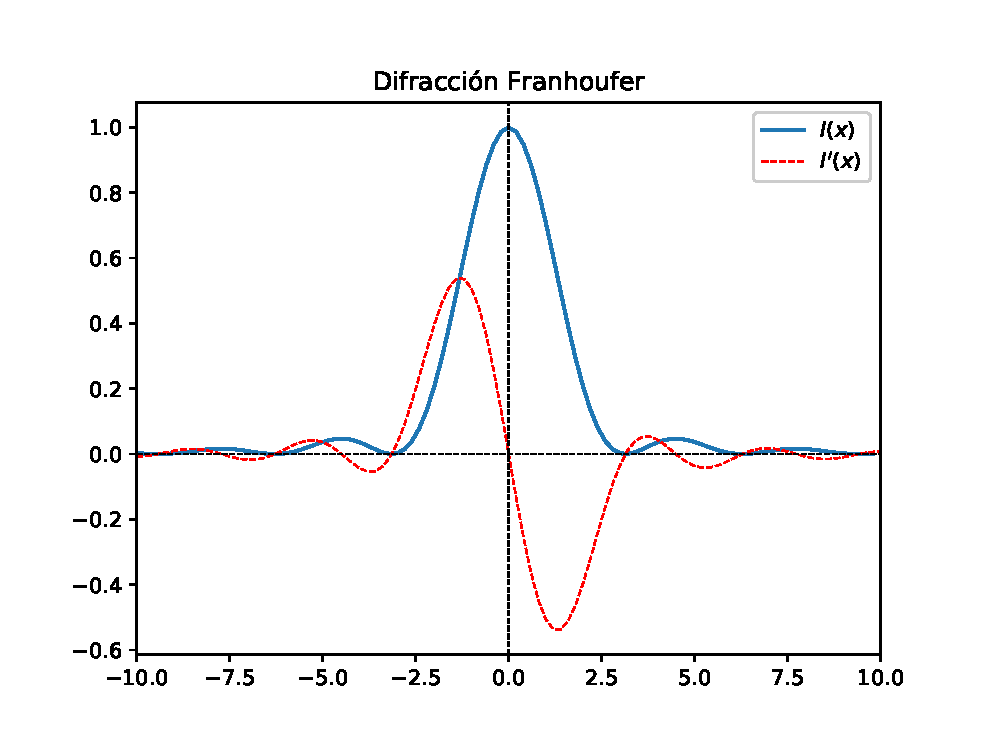
\includegraphics[scale=0.4]{Imagenes/raices_scipy_Franhoufer_01.eps}
    \caption{Detalle de la función y su derivada.}
\end{figure}
\end{frame}
\begin{frame}
\frametitle{Solución al ejercicio}
El programa debe de mostrar el valor del ancho medio $x_{1/2}$, los valores de intensidad máxima $x_{i}$, así como la gráfica solicitada.
\\
\bigskip
Las rutinas para el método de la secante y de la falsa posición ya se han revisado, sólo ajusta los argumentos; incluye las rutinas en un módulo \funcionazul{ModuloRaices.py}
\end{frame}
\end{document}